As said in the introduction, any cell of $\mathcal{C}$ can be
characterized as a point with integer coordinates, aka \emph{lattice
point}. A standard way is to double the coordinates of
the centroid of the cell (often called its Khalimsky code). Now we
have to represent an arbitrary set $K$ of lattice points.

Let $(\ve_j)_{j=1,\dots,d}$ be the canonical basis of $\Z^d$. We may
choose an arbitrary projection \emph{axis} $j \in
\{1,\ldots,d\}$. Letting $\pi_j$ be the projector along this axis, we
can collect all the cells of $K$ that projects onto the same
points. \replaced[id=ROM]{Consider a point}{Let} $p \in K$. Then $\pi^{-1}_j( \pi_j(p)) \cap \Star{K}$ is a set of cells having
all the same coordinates except along coordinate $j$. This set can be
ordered increasingly and stored as a list of integer intervals (see
Figure~\ref{fig:lattice-representation} for an illustration).

\begin{figure*}[t]
    \centering
    \newcommand{\drawBigRedSquare}[2]{% 2-cell red outline
    \draw[thick, red] (#1+1.1,#2+2.1) -- (#1+1.9,#2+2.1) -- (#1+1.9,#2+2.9) -- (#1+1.1,#2+2.9) -- cycle}
\newcommand{\drawBigRedVLine}[2]{% vertical 1-cell red outline
    \draw[thick, red] (#1+1,#2+2.1) -- (#1+1,#2+2.9)}
\newcommand{\drawBigRedHLine}[2]{% horizontal 1-cell red outline
    \draw[thick, red] (#1+1.1,#2+2) -- (#1+1.9,#2+2)}
\newcommand{\drawRedPoint}[2]{% 0-cell red dot
    \filldraw[thick, red] (#1,#2) circle (0.05)}
\newcommand{\drawKSquare}[2]{% 2-cell as black dot in Khalimsky coords
    \filldraw[black] (#1+1.5,#2+2.5) circle (0.05);}
\newcommand{\drawKVLine}[2]{% vertical 1-cell as black dot
    \filldraw[black] (#1+1,#2+2.5) circle (0.05);}
\newcommand{\drawKHLine}[2]{% horizontal 1-cell as black dot
    \filldraw[black] (#1+1.5,#2+2) circle (0.05);}
\newcommand{\drawKPoint}[2]{% 0-cell as black dot
    \filldraw[black] (#1,#2) circle (0.05);}
%%
\newcommand{\drawShapePoints}{%
    \filldraw[black] (1,4) circle (0.05);
    \filldraw[black] (1,5) circle (0.05);
    \filldraw[black] (2,5) circle (0.05);
    \filldraw[black] (3,5) circle (0.05);
    \filldraw[black] (3,4) circle (0.05);
    \filldraw[black] (3,3) circle (0.05);
    \filldraw[black] (3,2) circle (0.05);
    \filldraw[black] (2,2) circle (0.05);
    \filldraw[black] (1,2) circle (0.05);
    \filldraw[black] (4,2) circle (0.05);
}
\newcommand{\drawShapeCurve}{%
    \draw[black] (1,4) -- (1,5) -- (3,5) -- (3,2) -- (4,2) -- (1,2);
}
\newcommand{\drawStarBoundary}{%
    \draw[thick,dashed] (0,3) -- (0,1) -- (5,1) -- (5,3) -- (4,3) -- (4,6) -- (0,6) -- (0,3) -- (2,3) -- (2,4);
}
\newcommand{\drawAxesInteger}{%
    \draw[-{Stealth[length=3mm]}=black] (-1,0) -- (-1,7);
    \draw decorate [decoration={crosses,transform={rotate=45},shape size=1.5mm,segment length=15.6pt}] {(-1,1) -- (-1,6)};
    \foreach \y in {0,1,2,3,4,5} {
        \node at (-1.3,\y+1) {\scriptsize\y};
    }
    \draw[-{Stealth[length=3mm]}=black] (-1,0) -- (6.5,0);
    \draw decorate [decoration={crosses,transform={rotate=45},shape size=1.5mm,segment length=15.6pt}] {(-1,0) -- (5,0)};
    \foreach \x in {0,1,2,3,4,5} {
        \node at (\x,-0.5) {\scriptsize\x};
    }
}
\newcommand{\drawAxesKhalimsky}{%
    \draw[-{Stealth[length=3mm]}=black] (-1,0) -- (-1,7);
    \draw decorate [decoration={crosses,transform={rotate=45},shape size=1.5mm,segment length=7.8pt}] {(-1,1) -- (-1,6)};
    \foreach \y in {0,1,...,10} {
        \node at (-1.5,\y/2+1) {\scriptsize\y};
    }
    \draw[-{Stealth[length=3mm]}=black] (-1,0) -- (6.5,0);
    \draw decorate [decoration={crosses,transform={rotate=45},shape size=1.5mm,segment length=7.8pt}] {(-1,0) -- (5,0)};
    \foreach \x in {0,1,...,10} {
        \node at (\x/2,-0.5) {\scriptsize\x};
    }
}
\newcommand{\drawAllBigSquares}{%
    \drawBigRedSquare{-1}{-1};
    \drawBigRedSquare{-1}{0};
    \drawBigRedSquare{-1}{1};
    \drawBigRedSquare{-1}{2};
    \drawBigRedSquare{-1}{3};
    \drawBigRedSquare{0}{-1};
    \drawBigRedSquare{0}{0};
    \drawBigRedSquare{0}{1};
    \drawBigRedSquare{0}{2};
    \drawBigRedSquare{0}{3};
    \drawBigRedSquare{1}{-1};
    \drawBigRedSquare{1}{0};
    \drawBigRedSquare{1}{1};
    \drawBigRedSquare{1}{2};
    \drawBigRedSquare{1}{3};
    \drawBigRedSquare{2}{-1};
    \drawBigRedSquare{2}{0};
    \drawBigRedSquare{2}{1};
    \drawBigRedSquare{2}{2};
    \drawBigRedSquare{2}{3};
    \drawBigRedSquare{3}{-1};
    \drawBigRedSquare{3}{0};
}
\newcommand{\drawAllBigVLines}{%
    \drawBigRedVLine{0}{-1};
    \drawBigRedVLine{0}{0};
    \drawBigRedVLine{0}{1};
    \drawBigRedVLine{0}{2};
    \drawBigRedVLine{0}{3};
    \drawBigRedVLine{1}{-1};
    \drawBigRedVLine{1}{0};
    \drawBigRedVLine{1}{2};
    \drawBigRedVLine{1}{3};
    \drawBigRedVLine{2}{-1};
    \drawBigRedVLine{2}{0};
    \drawBigRedVLine{2}{1};
    \drawBigRedVLine{2}{2};
    \drawBigRedVLine{2}{3};
    \drawBigRedVLine{3}{-1};
    \drawBigRedVLine{3}{0};
}
\newcommand{\drawAllBigHLines}{%
    \drawBigRedHLine{-1}{0};
    \drawBigRedHLine{-1}{2};
    \drawBigRedHLine{-1}{3};
    \drawBigRedHLine{0}{0};
    \drawBigRedHLine{0}{2};
    \drawBigRedHLine{0}{3};
    \drawBigRedHLine{1}{0};
    \drawBigRedHLine{1}{1};
    \drawBigRedHLine{1}{2};
    \drawBigRedHLine{1}{3};
    \drawBigRedHLine{2}{0};
    \drawBigRedHLine{2}{1};
    \drawBigRedHLine{2}{2};
    \drawBigRedHLine{2}{3};
    \drawBigRedHLine{3}{0};
}
\newcommand{\drawAllRedPoints}{%
    \drawRedPoint{1}{4};
    \drawRedPoint{1}{5};
    \drawRedPoint{2}{5};
    \drawRedPoint{3}{5};
    \drawRedPoint{3}{4};
    \drawRedPoint{3}{3};
    \drawRedPoint{3}{2};
    \drawRedPoint{2}{2};
    \drawRedPoint{1}{2};
    \drawRedPoint{4}{2};
}
\newcommand{\drawAllKSquares}{%
    \drawKSquare{-1}{-1};
    \drawKSquare{-1}{0};
    \drawKSquare{-1}{1};
    \drawKSquare{-1}{2};
    \drawKSquare{-1}{3};
    \drawKSquare{0}{-1};
    \drawKSquare{0}{0};
    \drawKSquare{0}{1};
    \drawKSquare{0}{2};
    \drawKSquare{0}{3};
    \drawKSquare{1}{-1};
    \drawKSquare{1}{0};
    \drawKSquare{1}{1};
    \drawKSquare{1}{2};
    \drawKSquare{1}{3};
    \drawKSquare{2}{-1};
    \drawKSquare{2}{0};
    \drawKSquare{2}{1};
    \drawKSquare{2}{2};
    \drawKSquare{2}{3};
    \drawKSquare{3}{-1};
    \drawKSquare{3}{0};
}
\newcommand{\drawAllKVLines}{%
    \drawKVLine{0}{-1};
    \drawKVLine{0}{0};
    \drawKVLine{0}{1};
    \drawKVLine{0}{2};
    \drawKVLine{0}{3};
    \drawKVLine{1}{-1};
    \drawKVLine{1}{0};
    \drawKVLine{1}{2};
    \drawKVLine{1}{3};
    \drawKVLine{2}{-1};
    \drawKVLine{2}{0};
    \drawKVLine{2}{1};
    \drawKVLine{2}{2};
    \drawKVLine{2}{3};
    \drawKVLine{3}{-1};
    \drawKVLine{3}{0};
}
\newcommand{\drawAllKHLines}{%
    \drawKHLine{-1}{0};
    \drawKHLine{-1}{2};
    \drawKHLine{-1}{3};
    \drawKHLine{0}{0};
    \drawKHLine{0}{2};
    \drawKHLine{0}{3};
    \drawKHLine{1}{0};
    \drawKHLine{1}{1};
    \drawKHLine{1}{2};
    \drawKHLine{1}{3};
    \drawKHLine{2}{0};
    \drawKHLine{2}{1};
    \drawKHLine{2}{2};
    \drawKHLine{2}{3};
    \drawKHLine{3}{0};
}
\newcommand{\drawAllKPoints}{%
    \drawKPoint{1}{4};
    \drawKPoint{1}{5};
    \drawKPoint{2}{5};
    \drawKPoint{3}{5};
    \drawKPoint{3}{4};
    \drawKPoint{3}{3};
    \drawKPoint{3}{2};
    \drawKPoint{2}{2};
    \drawKPoint{1}{2};
    \drawKPoint{4}{2};
}
\begin{tabular}{c@{\hspace{4mm}}c}
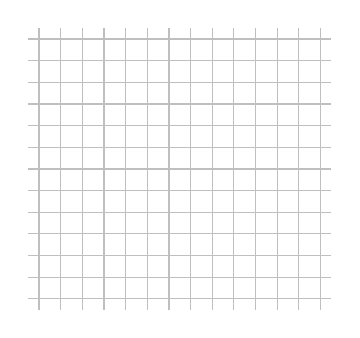
\begin{tikzpicture}[scale=0.55]
    \draw[step=0.5,lightgray,thin,xshift=-1cm,yshift=-1cm] (-0.25,0.75) grid (6.75,7.25);
    \drawAxesInteger
    \drawShapePoints
    \drawShapeCurve
    \drawStarBoundary
\end{tikzpicture}
&
\begin{tikzpicture}[scale=0.55]
    \draw[step=0.5,lightgray,thin,xshift=-1cm,yshift=-1cm] (-0.25,0.75) grid (6.75,7.25);
    \drawAxesInteger
    \drawShapeCurve
    \drawStarBoundary
    \drawAllBigSquares
    \drawAllBigVLines
    \drawAllBigHLines
    \drawAllRedPoints
\end{tikzpicture}
\\[-2mm]
\small (a) $Z$ and boundary of $\Star{Z}$ (dashed)
&
\small (b) Cells of $\Star{Z}$ in red
\\[4mm]
\begin{tikzpicture}[scale=0.55]
    \draw[step=0.5,lightgray,thin,xshift=-1cm,yshift=-1cm] (-0.25,0.75) grid (6.75,7.25);
    \drawAxesKhalimsky
    \drawShapeCurve
    \drawStarBoundary
    \drawAllBigSquares
    \drawAllBigVLines
    \drawAllBigHLines
    \drawAllRedPoints
    \drawAllKSquares
    \drawAllKVLines
    \drawAllKHLines
    \drawAllKPoints
\end{tikzpicture}
&
\begin{tikzpicture}[scale=0.55]
    \foreach \y in {2,2.5,...,7} {
        \draw[thin, lightgray,xshift=-1cm,yshift=-1cm] (-0.25,\y) -- (7.25,\y);
    }
    \draw[-{Stealth[length=3mm]}=black] (-1,0) -- (-1,7);
    \draw decorate [decoration={crosses,transform={rotate=45},shape size=1.5mm,segment length=7.8pt}] {(-1,1) -- (-1,6)};
    \foreach \y in {0,1,...,10} {
        \node at (-1.5,\y/2+1) {\scriptsize\y};
    }
    \drawStarBoundary
    \draw[thick, arrows = {Bracket[sharp]-Bracket[sharp]}] (0.4,5.5)--(3.6,5.5);
    \draw[thick, arrows = {Bracket[sharp]-Bracket[sharp]}] (0.4,5)--(3.6,5);
    \draw[thick, arrows = {Bracket[sharp]-Bracket[sharp]}] (0.4,4.5)--(3.6,4.5);
    \draw[thick, arrows = {Bracket[sharp]-Bracket[sharp]}] (0.4,4)--(1.6,4);
    \draw[thick, arrows = {Bracket[sharp]-Bracket[sharp]}] (2.4,4)--(3.6,4);
    \draw[thick, arrows = {Bracket[sharp]-Bracket[sharp]}] (0.4,3.5)--(1.6,3.5);
    \draw[thick, arrows = {Bracket[sharp]-Bracket[sharp]}] (2.4,3.5)--(3.6,3.5);
    \draw[thick, arrows = {Bracket[sharp]-Bracket[sharp]}] (2.4,3)--(3.6,3);
    \draw[thick, arrows = {Bracket[sharp]-Bracket[sharp]}] (0.4,2.5)--(4.6,2.5);
    \draw[thick, arrows = {Bracket[sharp]-Bracket[sharp]}] (0.4,2)--(4.6,2);
    \draw[thick, arrows = {Bracket[sharp]-Bracket[sharp]}] (0.4,1.5)--(4.6,1.5);
    \node at (0,-0.5) {};
\end{tikzpicture}
\\[-2mm]
\small (c) Khalimsky coding (each $\bullet$ encodes a cell)
&
\small (d) Lattice map (11 intervals)
\end{tabular}

    \caption{\label{fig:lattice-representation} \replaced[id=ROM]{Representation of a
    2d cell complex (here the star of a given curve) as a lattice
    map. (a)~The digital set $Z$ (black dots $\bullet$) and the
    boundary of $\Star{Z}$ (dashed). (b)~The cells of $\Star{Z}$
    shown in red: 2-cells (squares), 1-cells (segments), and 0-cells
    (dots). (c)~Khalimsky coding: each of the 63 cells is encoded as
    a lattice point with doubled coordinates (black $\bullet$); each
    red outline shows the original cell it encodes. (d)~Projection
    along one axis yields a lattice map of 11 integer intervals.}{Representation of a
    2d cell complex (here the star of a given curve) as a lattice
    map. From 63 cells (with two coordinates) on the top, we get 11
    intervals on the bottom.}}
\end{figure*}


A \emph{sequence of intervals} is an ordered list of intervals $L =
([a_i,b_i])_{i=1,\ldots,n}$ such that $a_i \in \Z, b_i \in \Z, b_i + 1
< a_{i+1}$, i.e., disjoint intervals with at least a missing
integer. We denote by $\mathbb{L}$ the set of sequences of
intervals. An integer $k$ belongs to $L$ iff there exists $i$ such that
$a_i \Le k \Le b_i$. For a finite set of integers, there is a unique
sequence of intervals representing it.

A \emph{lattice map along axis $j$} is a set of pairs $(q,L_q)$, with
$q \in \Z^{d-1}$ and $L_q \in \mathbb{L}$. The lattice map $M_K$
\emph{represents} $K$ when, for any point $p \in K$, the pair
$(\pi_j(p), L_{\pi_j(p)})$ exists in $M_K$ and $p_j \in L_{\pi_j(p)}$,
with $p_j$ the $j$-th coordinate of $p$, and reciprocally, $\forall
(q,L_q) \in M_K, \forall i \in L_q, q+i\ve_j \in K$. A lattice map is
thus made of pairs $(q,L_q)$, where $q$ is the \emph{shift} while
$L_q$ is the \emph{intervals}. For a point $q$ which is a shift of
$M_K$, we write $M_K[q]$ for the corresponding intervals $L_q$.

The global algorithm for computing visibility is given in
Algorithm~\ref{alg:visibility}. Given a digital input surface $C$ (a
subcomplex), we compute the lattice map $\Omega$ of $\Star{C}$ once,
generally along the axis where $C$ is the most elongated. In order to
compute visibility up to a given distance $r$, we consider all
non-null primitive vectors $D$ with infinity norm no greater than $r$.
For each vector $\vv$, we compute the lattice map $M_\vv$ of the cells
intersected by the vector from $\mathbf{0}$ to $\vv$ in $\R^d$
(see \RefFigure{fig:visibility-algorithm-evolution}, top-right). The
visibility along the direction $\vv$ reduces to computing for each
pair of $M_\vv$ the possible translations of intervals in $\Omega$,
and then intersecting all the translations.

%% \begin{definition}
%%   A sequence of intervals is an ordered list of intervals $L = ([a_i,b_i])_{i=1,\ldots,n}$ such that $b_i + 1 < a_{i+1}$, i.e., disjoint intervals with at least a missing integer.
%% \end{definition}

%% \begin{definition}
%%   A translation of an interval $A$ is defined as $A+t \coloneqq [a+t, b+t]$
%% \end{definition}

%% \begin{definition}
%%   A translation of a sequence of intervals $L$ is the sequence defined as $L+t \coloneqq \{L_1+t,\ldots,L_n+t\}$
%% \end{definition}

%% \begin{definition}
%%   All translations $T$ of an interval or a sequence of intervals $A$ in a sequence of intervals $L$ are defined as $ T \coloneqq \{ t, st. A+t \subset L\}$
%% \end{definition}

%% We will consider lattice maps as pairs of (shift, intervals), where shifts are points $p \in \R^{d-1}$. All coordinates are doubled, so that the represented cell $\forall c \in \R^d$ will have a dimension equal to $\sum_{i=1}^d \left(c[i]\mod d\right)$.
%% In figure~\ref{fig:lattice-representation}, we display a representation of lattice maps applied to a 2-d cell complex where all coordinates are already doubled. Note that the examples are in 2-d, the shown results are in 3-d and the algorithm is for n-d.


\begin{algorithm*}
    \caption{Given a subcomplex $C$ and an integer $r$, returns the visibility from every point of $C$ up to distance $r$. The main axis is supposed to be $z$, while $x,y$ are the auxiliary axes.}
    \label{alg:visibility}
    \begin{algorithmic}
        \Function{Visibility}{$C$: Subcomplex, $r$: Integer}
            \State $\Omega \gets M_{\Call{Star}{C}}$ \Comment{Lattice map of the star of input subcomplex}
            \State $Directions \gets \Call{GetAllPrimalDirections}{r}$
            \State $V: \text{vector of boolean} \gets [0, \ldots, 0]$ \Comment{length $Size(Directions) \times \#C.pointels$}
            \State $low, high \gets \Call{BoundingBoxZ}{\Omega}$
            \ForAll{$\vv$ in $Directions$}
                \ForAll{shift $S$ in $\Omega$}
                    \State $R \gets [low, high]$
                    \ForAll{pair $P$ in $M_{\Call{Star}{[\mathbf{0},\mathbf{v}]}}$}
                        \State $R \gets R \cap \Call{Translations}{P.intervals,\Omega[S + P.shift]}$
                    \EndFor
                    \State \Call{UpdateVisibility}{$V$, $R$}
                \EndFor
            \EndFor
            \State \Return $V$
        \EndFunction
    \end{algorithmic}
\end{algorithm*}


\begin{figure*}
    \centering
    \input{algorithm.tikz}
    \caption{Evolution of the visibility check algorithm for a $(2,1)$
        vector. \replaced[id=ROM]{The vector lattice map is in green, the figure
        lattice map is in black and the current intervals of positions where
        the visibility is still possible are in red.}{Green is the vector lattice map, black is the figure
        lattice map, red are the current intervals of positions where
        the visibility is still possible.} The last red intervals are
        the visible positions. We travel the lattice maps from
        bottom-up and the found visibilities are drawn on the
        uppermost figure.}
    \label{fig:visibility-algorithm-evolution}
\end{figure*}

\added[id=ROM]{Figure~\ref{fig:visibility-algorithm-evolution} illustrates the
execution of Algorithm~\ref{alg:visibility} on an elementary 2D
example, for the direction vector $\vv=(2,1)$.  The top-left part~(F)
shows the digital set $Z$ (black dots and bold edges) together with
its star $\Star{Z}$, whose boundary is drawn as a dashed outline. The
star is projected along the chosen main axis (here the vertical axis),
yielding the \emph{figure lattice map} $\Omega$: the gray bracket
intervals on the right of~(F), organized by row number $1,\ldots,5$
from bottom to top.  The top-right part~(V) shows the direction vector
$\vv$ from $\mathbf{0}$ to $(2,1)$ together with its star
$\Star{[\mathbf{0},\vv]}$, projected along the same axis into the
\emph{vector lattice map} $M_\vv$: the green bracket intervals,
again organized by row.}

\added[id=ROM]{The bottom part details the core computation, which processes each
projected row (shift) $i=1,\ldots,5$ in sequence. For each row~$i$:}
\begin{enumerate}
  \item \added[id=ROM]{$V_i$ (green interval) is the entry of the vector lattice map
    $M_\vv$ at row~$i$.}
  \item \added[id=ROM]{$F_i$ (gray intervals) is the entry of the figure lattice map
    $\Omega$ at the corresponding shifted row $S + P.\mathrm{shift}$.}
  \item \added[id=ROM]{$T_i$ (violet intervals) is the set of all translations~$t$
    such that $V_i + t \subseteq F_i$, i.e., all positions where the
    green interval fits entirely inside the gray intervals.}
  \item \added[id=ROM]{$R_i$ (red intervals) is the current intersection: $R_1 = T_1$
    and $R_i = T_i \cap R_{i-1}$ for $i \geq 2$.  The black dots on
    $R_i$ mark the integer positions within these intervals.}
\end{enumerate}
\added[id=ROM]{When a row of the vector lattice map is offset along the auxiliary axis
(as for rows~4 and~5 where $V_i$ starts at a shifted position,
indicated by the black arrow), the corresponding figure intervals
$F_i$ are looked up at the appropriately shifted key in $\Omega$.}

\added[id=ROM]{After all rows have been processed, the final result $R_5$ gives all
starting positions~$t$ along the auxiliary axis where the entire
translated set $\Star{[\mathbf{0},\vv]}+t$ fits inside
$\Star{Z}$.  Each such integer position~$t$ corresponds to a pair of
points $(p, p+\vv)$ that are visible in~$Z$.  These pairs are drawn as
red arrows on the top-left figure~(F).  Note that the process can be
stopped early as soon as the current intersection $R_i$ becomes empty,
since further intersections cannot produce new positions.
This procedure requires a data representation that is both compact in
storage and efficient for the interval inclusion and intersection
operations at its core.  Lattice maps fulfill both requirements: they
encode a potentially large cell complex as a small collection of
integer interval sequences, and all the key operations
(translation, inclusion test, intersection) reduce to simple
linear-time scans over sorted intervals.}

\replaced[id=ROM]{In general, the algorithm reduces to determining all possible
inclusions by translation of sequences of intervals into another
sequence of intervals (note that for pairwise visibility, it is enough
to consider all possible inclusions by translation of \emph{one} interval
into another sequence of intervals), and then intersecting
progressively the results. Some results of visible points are
displayed on Figure~\ref{fig:visibility-results} on 3D shapes.}{Figure~\ref{fig:visibility-algorithm-evolution} shows an example of
execution of this algorithm in an elementary case. It reduces to
determining all the possible inclusions by translation of sequences of
intervals in another sequence of intervals (note that for
pairwise visibility, it is enough to consider all the possible
inclusions by translation of one interval in another sequence of
intervals), and then intersecting progressively the results. Of
course, the process is stopped as soon as the intersection is
empty. Some results of visible points are displayed on
figure~\ref{fig:visibility-results} on 3d shapes.}

%% In order to compute the visibility, we first compute $\Omega = \text{Star}(C)$. Then for each primal direction of
%% coordinates at most $r$, we look at all the possible positions this specific direction does link 2 visible points
%% of the cell complex. In order to do so, for each shift in $\Omega$, we compute the positions where points are
%% visible using the same method as presented in~\ref{fig:visibility-algorithm-evolution}. Some results of visible
%% points are present in figure~\ref{fig:visibility-results}.

\begin{algorithm}
    \caption{Given 2 lists of integer intervals $K$ and $L$, returns $K \cap L$}
    \label{alg:intersection}
    \begin{algorithmic}
        \Function{Intersection ($\cap$)}{\text{K, L}: Intervals}
            \State $R \gets \emptyset$; $k \gets 0$; $l \gets 0$;
            \While{$k < K.size \And l < L.size$}
                \State $[a,b] \gets K[k]$; $[c,d] \gets L[l]$
                \State $e \gets \max(a, c)$; $f \gets \min(b, d)$;
                \If{$e \leq f$}
                    $R.append([e, f])$;
                \EndIf
                \If{$b \leq d$}
                    $k \gets k+1$;
                \EndIf
                \If{$d \leq b$}
                    $l \gets l+1$;
                \EndIf
            \EndWhile
            \State \Return $R$
        \EndFunction
    \end{algorithmic}
\end{algorithm}

To efficiently compute the intersection of two sequences of intervals
$K$ and $L$ (Algorithm~\ref{alg:intersection}), we go through the
first two unvisited elements of the two lists. If they do not overlap
(i.e.\ the start and end of the \replaced[id=ROM]{first}{1st} interval are both smaller than the
start of the other), then we can discard the smaller interval. Else,
we output the intersection of these 2 intervals as one of the
resulting intervals. We then skip the interval with the smallest
end. If both intervals have the same end, then both intervals can be
skipped. Doing this computation until one of the two lists is empty
returns the intersection of the input two lists of intervals.

\begin{figure}
    \centering
    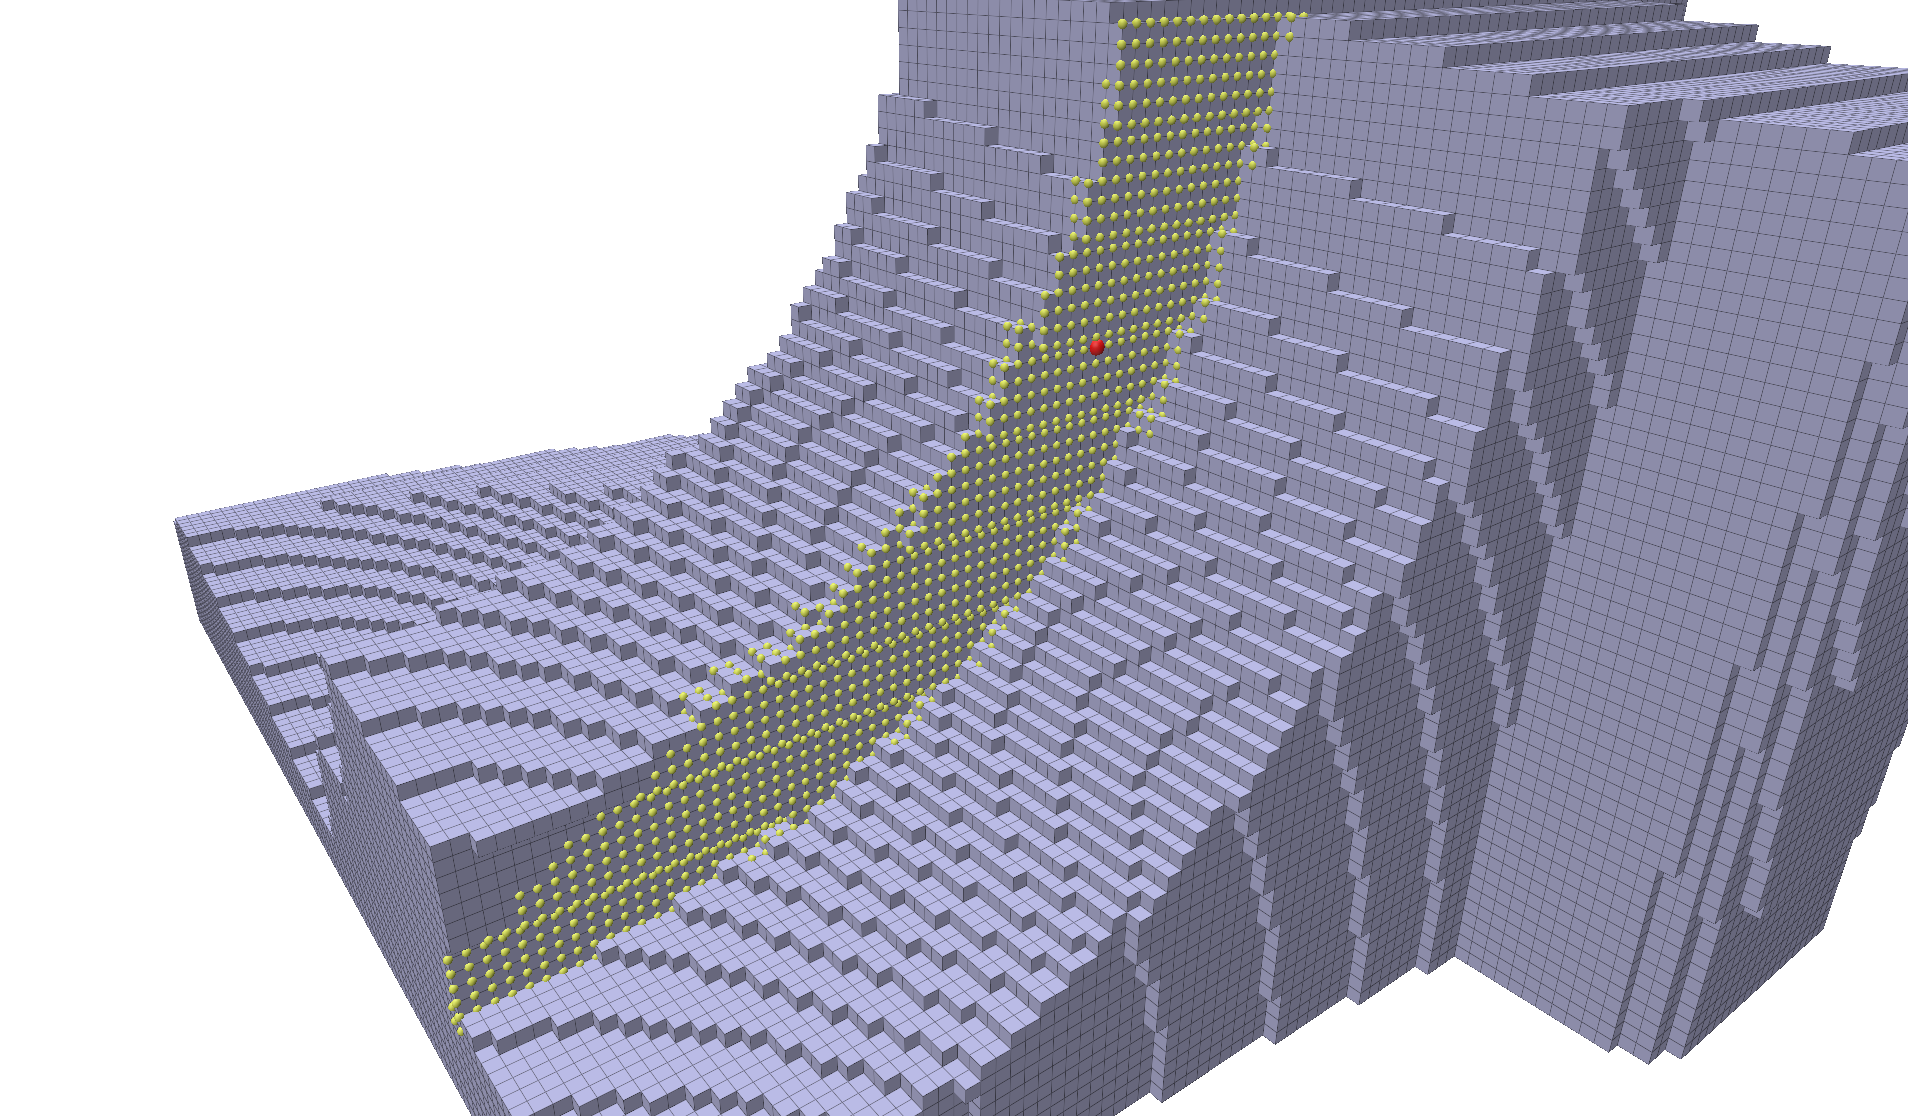
\includegraphics[width=0.85\columnwidth]{pictures/visibility_aware_of_saillencies}\\[6pt]
    
\includegraphics[width=0.85\columnwidth]{pictures/visibility_aware_of_features}
    \caption{\replaced[id=ROM]{Examples of visibilities from a source
    point. (a)~On a fandisk, the visibility is stopped at the sharp
    edge. (b)~On a torus knot, the visibility does not cross the gap
    between the two parts.}{Examples of visibilities from a source point:
        (top) the visibility is stopped at the sharp edge, (bottom) the
        visibility does not cross the gap between the two parts.}}
    \label{fig:visibility-results}
\end{figure}
%
%    \begin{figure*}
%        \begin{center}
%            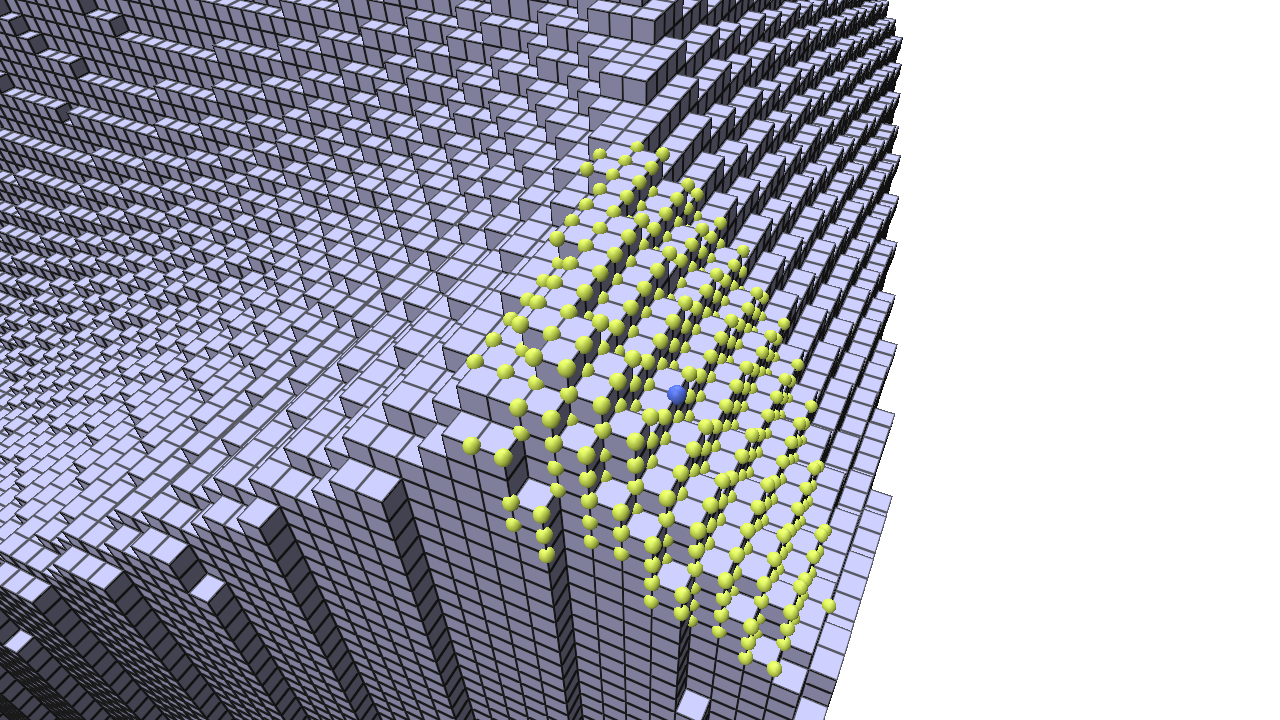
\includegraphics[width=0.8\textwidth]{pictures/visibility_from_given_point_r_10}
%            \caption{Visibility of a point on an edge of a fandisk}
%            \label{fig:visibility-fandisk}
%        \end{center}
%    \end{figure*}
%    \begin{figure*}
%        \begin{center}
%            
\includegraphics[width=0.8\textwidth]{pictures/visibility_aware_of_features}
%            \caption{Visibility of a point on a torus knot (the visibility is feature-aware)}
%            \label{fig:visibility-torus-knot}
%        \end{center}
%    \end{figure*}


% Quantitative results

We have plotted on
Figure~\ref{fig:meanvisibility-computationComplexity} the running
times to compute global visibility of both~\cite[Algorithm
3]{lachaud:2022-jmiv} and our algorithm. Timings are very similar. Our
algorithm is faster for smaller maximal radii (up to 20), while the
other is slightly faster for bigger radii. We have also measured the
discrete average visibility distance along digitization of smooth
shapes for $\Starop_1$ (Figure~\ref{fig:meanvisibility-gridstep}).
Smooth shapes studied are sphere9 (or Sphere) ($x^2+y^2+z^2=81$), goursat ($0.03\left(x^4+y^4+z^4\right)-2\left(x^2+y^2+z^2\right)=8$),
torus ($\left(x^2+y^2+z^2+32\right)^2-144\left(x^2+y^2\right)=0$), leopold ($x^2 y^2 z^2+4\left(x^2+y^2+z^2\right)=100$)
and rcube (or Rounded Cube) ($x^4+y^4+z^4=6561$). Most of the shapes follows
a law in $\Theta\left( h^{-\frac{1}{2}} \right)$, excepted rcube and leopold,
which contains flat surfaces which makes the visibility distance grow faster
than the previous law (measured to be between $\Theta\left( h^{-\frac{3}{5}} \right)$
and $\Theta\left( h^{-\frac{2}{3}} \right)$).

We have also tested the average visibility distance on a GluedEllipsoid with $\Starop_1$ and $\Starop_2$
(Figure~\ref{fig:meanvisibility-gridstep-piecewise}). Both $\Starop$ follow a law
proportional to $h^{-\frac{1}{2}}$, but $\Starop_2$ has a bigger constant.
Thus, the average continuous visibility distance is proportional
to $\sqrt{h}$. As shown in the next section, for real 3d images,
a maximal radius below 10 is sufficient for normal and curvature estimation.

\begin{figure}[t]
    \centering
    \input{pointelscomptime.tikz}
    \caption{ \label{fig:meanvisibility-computationComplexity}Computation
    time of visibility as a function of the number of pointels. We
    compare the running time of the naive breadth first visibility
    algorithm against our algorithm using intervals. We input the same
    maximal radius to both versions (10, 20, 30) and test it on 6
    different figures (goursat, torus, rcube, sphere9, leopold,
        ``D20'') with various gridsteps, ($\#$ pointels ranging from 520
        to 390235).}
\end{figure}

\begin{figure}
    \centering
    \input{mean-distance.tikz}
    \caption{\label{fig:meanvisibility-gridstep} Mean discrete distance of visibility as a function of the gridstep $h$ (see text).}
\end{figure}

\begin{figure}
    \centering
    \input{mean-distance-piecewise.tikz}
    \caption{\label{fig:meanvisibility-gridstep-piecewise} Mean discrete distance of visibility as a function of the gridstep $h$ for the piecewise smooth shape GluedEllipsoid (see text).}
\end{figure}
